 % % % % % % % % % % % % % % % % % % % % % % % % % % % % % % % % % % % %
 % % % % % % % % % % % % % % % % % % % % % % % % % % % % % % % % % % % %
 % % % % % % % % % % % % % % % % % % % % % % % % % % % % % % % % % % % %

\documentclass[paper=a4, fontsize=11pt]{scrartcl} 
\usepackage[T1]{fontenc} 
\usepackage{fourier} 
\usepackage{graphicx}
\usepackage[english]{babel} 
\usepackage{amsmath,amsfonts,amsthm} 
\usepackage{listings}
\usepackage{sectsty} 
\allsectionsfont{\centering \normalfont\scshape} 
\usepackage{fancyhdr} % Custom headers and footers

 % % % % % % % % % % % % % % % % % % % % % % % % % % % % % % % % % % % %

\pagestyle{fancyplain} 
\fancyhead{} 
\fancyfoot[L]{} 
\fancyfoot[C]{} 
\fancyfoot[R]{\thepage} 
\renewcommand{\headrulewidth}{0pt} 
\renewcommand{\footrulewidth}{0pt} 
\setlength{\headheight}{13.6pt} 
\numberwithin{equation}{section} 
\numberwithin{figure}{section} 
\numberwithin{table}{section}
\setlength\parindent{0pt} 

 % % % % % % % % % % % % % % % % % % % % % % % % % % % % % % % % % % % %

\newcommand{\horrule}[1]{\rule{\linewidth}{#1}}  
 
 % % % % % % % % % % % % % % % % % % % % % % % % % % % % % % % % % % % %

\title{	
\normalfont \normalsize 
\textsc{Barcelona Graduate School of Economics - Data Science} \\ [25pt]
\horrule{2pt} \\[0.5cm] 
\huge Deep Feature Learning for (Random) Forest Cover Type Prediction  \\ 
\horrule{2pt} \\[0.5cm] 
}


\author{J\'essica Leal, Tim Kreienkamp and Philipp Schmidt} 
\date{}



 % % % % % % % % % % % % % % % % % % % % % % % % % % % % % % % % % % % %


\begin{document}



 % % % % % % % % % % % % % % % % % % % % % % % % % % % % % % % % % % % %


\maketitle
\textbf{Abstract:} \\
From a seven-class training data with 50,000 observations we try to find the best predictive model using different Machine Learning algorithm such as K-nearest neighbors, GBM, Support Vector Machine, Random Forest and Random Forest with deep learning. Our aim is to best predict this seven-class data set with 100,000 observations. For each model, we perform a 10-fold cross validation in order to assess the performance of our classifier in the training data set. After estimating the best hyperparameters for each model - with cross-validation - and comparing the train performance, we consider the Random Forest with deep feature learning is the best type of algorithm which can predict better our data. 


 % % % % % % % % % % % % % % % % % % % % % % % % % % % % % % % % % % % %



\section{Introduction}
\subsection{Dataset Characteristics}
In this project, we work with a training data set of 50,000 observations - with labels - and a testing set - without labels - of 100,000 observations. Our aim is to predict a seven-class variable in which each label is a different type of forest cover using cartographic variables. We have 10 numeric variables presented in a raw manner that needed to be scaled, and 44 binary variables for qualitative aspects of the forest such as the wilderness of that forest and the type of soil. 

\newpage



 % % % % % % % % % % % % % % % % % % % % % % % % % % % % % % % % % % % %
\subsection{Baseline}
Before considering a unique and a priori thought best classifier, we attempted to model our data with different other classifier such as the K-NN and the SVM in order to mark us a benchmark for future steps in classification.


 % % % % % % % % % % % % % % % % % % % % % % % % % % % % % % % % % % % %

\section{Exploratory Analysis}



 % % % % % % % % % % % % % % % % % % % % % % % % % % % % % % % % % % % %


\section{Methods}
\subsection{K-Nearest Neighbor}
With this method, we try to classify each new observation in the test set taking into consideration the majority label from its the labels of its a certain number of nearest neighbors (K). In our case, we used the Euclidean distance as a measure of closeness between observations.


\subsection{Support Vector Machine}
This algorithm tries to predict the labels of the data set by separating the space into halfspaces - where in each halfspace we have a different label for the observations - with the largest margin (separation) possible. We can also introduce a cost parameter which tends to penalize the misclassification done within the bands. 

\subsection{Gradient Boosting}
This is an algorithm for predicting labels which combines different weak prediction models to create one which is strong, and in our case we used decision trees. So it tries to find the best algrotihm by weighting different functions. Those weights are updated considering the misclassifications. 

\subsection{Random Forest}
This method tries to create a strong classifier from the weighted sum of different decision trees. In each iteration it considers a random sample with replacement in the training set and fits a decision tree. Then, it considers a small subsets of the features, and we divide the space considering thevariable that best separates the space. We do this procedure for many iterations. 


\subsection{Random Forest with deep learning}
This  method tries to combine the benefits from the Random Forest with the benefits from Deep learning. It takes into account that the data might have some hidden layers that transform the data. 








 % % % % % % % % % % % % % % % % % % % % % % % % % % % % % % % % % % % %

\section{Experiments}
In a first set of experiments, we consider several well established classes of hypothesis functions. In particular, we consider Random Forests, Support Vector Machines, k-NN,  Gradient Tree Boosting and Neural Nets (Deep Learning). 
We first run these over a grid of hyperparameters without any feature engineering. This gives us a feeling for how well different methods are suited for the task at hand. In grid search, one evaluates a classifier over a grid, i.e. the cartesian product of several hyper parameter ranges. This process is computationally intensive, but since the data set is small, we can afford this luxury. The code for these experiments can be found in the files \lstinline{h2o_gridsearches.R}, \lstinline{svm_experiments.R} and \lstinline{knn_experiments.R}. The following figure shows the accuracy of the best model in each class. All accuracy values are obtained by a 10-fold cross validation procedure. 

\begin{figure}[p]
    \centering
    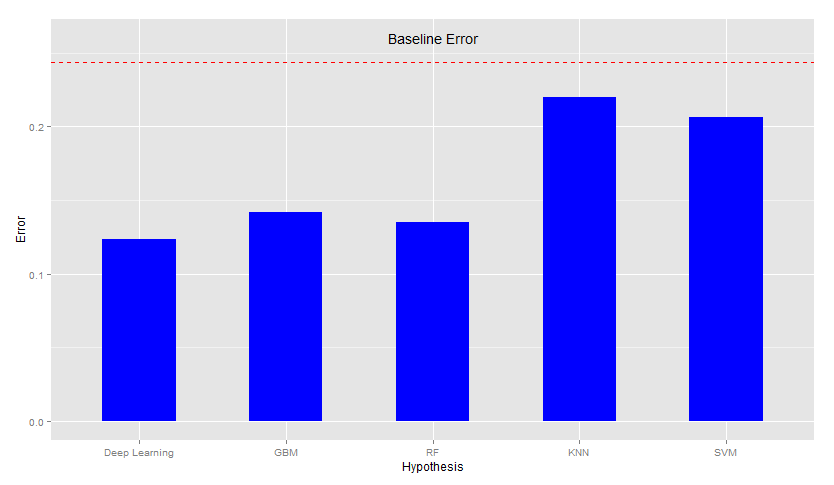
\includegraphics[width=0.8\textwidth]{erorrs.png}
    \caption{Initial errors with different methods}
    \label{fig:errors}
\end{figure}

We clearly see that the performance of SVM and k-NN, at least in the tried configuration with this set of features is rather disappointing. Tree based methods  and neural nets however, show - with some parameter tuning - a significant improvement over the baseline. 
 \newpage




DESCRIPTION OF PROCEDURE DONE WITH KNN
 In order to see which hyperparameter k we should use, we use 10-fold cross-validation with different values of k, and we see that considering the label from the training set as a factor or as an integer does not affect our results. The best value of K-NN which minimizes our cross-validation training error is 3. In the case in which Y is a factor, we get an error of 22.01\%; and when Y is an integer we get an error of 22.066\%. We consider the error is quite high in the training set, so this is one of the reasons why we decided to extend our models to take into account. 



DESCRIPTION OF PROCEDURE DONE WITH SVM
 The package used in this analysis was 'kernlab' with the function 'ksvm'. We decided to use spoc-svc type of classification which deals with multiclasses.  We tried different parameters for the cost parameters of the soft-margin SVM which tend to penalize the misclassification of the observatiosn, leading to a tradeoff of large margin and a small error penalty . The optimal cost to choose is 2. Using this classification we found that our cross-validation error was 20.62\%, which is still high. 



GRADIENT BOOSTING
The next method we wanted to try was the Gradient Boosting method\footnote{The package used is 'h2o'}. 
With this method we try to construct a classification tree of the labels why using one type of loss function, 
The CV error in this case is 14.154\% which is a great improvement from the previous methods, but it is still not low enough. 



 % % % % % % % % % % % % % % % % % % % % % % % % % % % % % % % % % % % %


\section{Feature Engineering and Model Tuning}
We settle on Deep Learning and Random Forests, since those performed best in the initial series of experiments. Based on our exploratory analysis, we add three new features to the data set: Horizontal Distance to Hydrology (water), Vertical Distance to Hydrology, and Total Distance to Hydrology. We feed these into the our previously best performing models, which leaves us with a slight gain in accuracy. 
Since Deep Learning seems to perform well for this data set, we try a heuristic: Why not train the Random Forest on features extracted with Deep Learning? The recent success on Deep Learning seems to be partly based on it's ability to abstract high-level concepts from the data. For this reason, Machine Learning researchers use it for feature, or representation learning. Feature learning can be done in a supervised or unsupervised manner. We use it in a supervised manner based on the heuristic: the neural net with the highest accuracy will provide the best features for our random forest. Operatively, what is done is just that the nodes of the last hidden layer in the neural net are extracted and used to transform the original feature space. The following figure shows the accuracy of all methods described: Random Forests, Deep Learning, and Random Forests with "Deep Features". 


We see that this results in a significant gain in accuracy. Apparently, Deep Learning is able to extract useful features from the data. However, in our last example we trained the random forest on 200 features. Too many features may potentially cause overfitting. This is why, in the next series of experiments, we add another layer to the neural net, where the size is significantly reduced, thus enforcing sparseness in the output. We try this with 50, 30 and 20 neurons. 


Inspecting the output shows that

 % % % % % % % % % % % % % % % % % % % % % % % % % % % % % % % % % % % %


\section{Limitations}
Some of the main limitations in this project are 

 % % % % % % % % % % % % % % % % % % % % % % % % % % % % % % % % % % % %

\section{Conclusions}

 % % % % % % % % % % % % % % % % % % % % % % % % % % % % % % % % % % % %


\end{document}
 % % % % % % % % % % % % % % % % % % % % % % % % % % % % % % % % % % % %
 % % % % % % % % % % % % % % % % % % % % % % % % % % % % % % % % % % % %
 % % % % % % % % % % % % % % % % % % % % % % % % % % % % % % % % % % % %
